\chapter{\sffamily Building a generalised simulator}

{\bfseries\sffamily Concept.} To design and build a generalised simulation engine that is able to generate samples from a `Pokédex' of possible stochastic processes that a researcher might encounter. A `Pokédex' here is just a fanciful description for a very general class of multidimensional stochastic processes that pop up everywhere in taming the mathematical wilds of real-world phenomena, and which also leads to a name for the software itself: the `stochadex'. With such a thing pre-built and self-contained, it can become the basis upon which to build generalised software solutions for a lot of different problems. For the mathematically-inclined, this chapter will require the introduction of a new formalism which we shall refer back to throughout the book. For the programmers, the public Git repository for the code that is described in this chapter can be found here: \href{https://github.com/umbralcalc/stochadex}{https://github.com/umbralcalc/stochadex}.

\section{\sffamily Computational formalism}

Before we dive into software design of the stochadex, we need to mathematically define the general computational approach that we're going to take. Because the language of stochastic processes is primarily mathematics, we'd argue this step is essential in enabling a really general description. From experience, it seems reasonable to start by writing down the following formula which describes iterating some arbitrary process forward in time (by one finite step) and adding a new row each to some matrix $X' \rightarrow X$
%%
\begin{align}
X^{i}_{{\sf t}+1} &= F^{i}_{{\sf t}+1}(X',{\sf t}) \,, \label{eq:x-step-def}
\end{align}
%%
where: $i$ is an index for the dimensions of the `state' space; ${\sf t}$ is the current time index for either a discrete-time process or some discrete approximation to a continuous-time process; $X$ is the next version of $X'$ after one timestep (and hence one new row has been added); and $F^i_{{\sf t}+1}(X',{\sf t})$ as the latest element of an arbitrary matrix-valued function. As we shall discuss shortly, $F^i_{{\sf t}+1}(X',{\sf t})$ may represent not just operations on deterministic variables, but also on stochastic ones. There is also no requirement for the function to be continuous.

\begin{figure}[h]
\centering
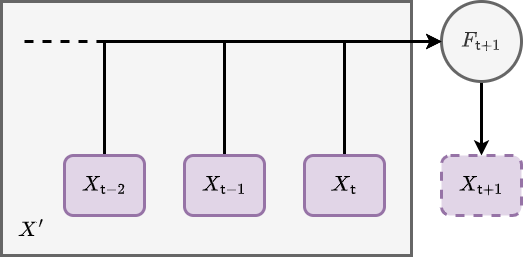
\includegraphics[width=10cm]{images/fundamental-loop.drawio.png}
\caption{Graph representation of Eq.~(\ref{eq:x-step-def}).}
\label{fig:fundamental-loop}
\end{figure}

The basic computational idea here is illustrated in Fig.~\ref{fig:fundamental-loop}; we iterate the matrix $X$ forward in time by a row, and use its previous version $X'$ as an entire matrix input into a function which populates the elements of its latest rows. In Go you could easily write something with the same idea in it, and the code would probably look like this.

\begin{lstlisting}[language=Go]
type StateVector  []float64
type StateHistory []StateVector

// iterate the state history forward in time by one step
func IterationFormula(
    stateHistory StateHistory, 
    timeStepNumber int,
) StateVector {
    for t, stateVector := range stateHistory {
        for i, stateElement := range stateVector {
            // do something
        }
    }
    return newestStateVector
}
\end{lstlisting}

Pretty simple! But why go to all this trouble of storing matrix inputs for previous values of the same process? It's true that this is mostly redundant for \emph{Markovian} phenomena, i.e., processes where their only memory of their history is the most recent value they took. However, for a large class of stochastic processes a full memory\footnote{Or memory at least within some window.} of past values is essential to consistently construct the sample paths moving forward. This is true in particular for \emph{non-Markovian} phenomena, where the latest values don't just depend on the immediately previous ones but can depend on values which occured much earlier in the process as well.

For more complex physical models and integrators, the distinct notions of `numerical timestep' and `total elapsed continuous time' will crop up quite frequently. Hence, before moving on further details, it will be important to define the total elapsed time variable $t({\sf t})$ for processes which are defined in continuous time. Assuming that we have already defined some function $\delta t({\sf t})$ which returns the specific change in continuous time that corresponds to the step ${\sf t}-1 \rightarrow {\sf t}$, we will always be able to compute the total elapsed time through the relation
%%
\begin{align}
t({\sf t}) &= \sum^{{\sf t}}_{{\sf t}'=0}\delta t({\sf t}') \label{eq:t-steps-sum} \,.
\end{align}
%%
This seems a lot of effort, no? Well it's important to remember that our steps in continuous time may not be constant, so by defining the $\delta t({\sf t})$ function and summing over it we can enable this flexibility in the computation. In case the summation notation is no fun for programmers; in Go we're implicitly doing this.

\begin{lstlisting}[language=Go]
// get the next increment from this step number forward in
// some unit of time, e.g., seconds
func TimeIncrementFunction(timeStepNumber int) float64 {
    // compute the next increment
    return nextTimeIncrement
}

// compute the total time elapsed up to the input step number in
// some unit of time, e.g., seconds
func ElapsedTimeFunction(timeStepNumber int) float64 {
    totalElapsedTime := 0.0
    for t := 0; t < timeStepNumber; t++ {
        totalElapsedTime += TimeIncrementFunction(t)
    }
    return totalElapsedTime
}
\end{lstlisting}

So, now that we've mathematically defined a really general notion of iterating the stochastic process forward in time, it makes sense to discuss some simple examples. For instance, it is frequently possible to split $F$ up into deteministic (denoted $D$) and stochastic (denoted $S$) matrix-valued functions like so
%%
\begin{align}
& F^{i}_{{\sf t}+1}(X',{\sf t}) = D^{i}_{{\sf t}+1}(X',{\sf t}) + S^{i}_{{\sf t}+1}(X',{\sf t}) \,.
\end{align}
%%
In the case of stochastic processes with continuous sample paths, it's also nearly always the case with mathematical models of real-world systems that the deterministic part will at least contain the term $D^{i}_{{\sf t}+1}(X',{\sf t}) = X^i_{\sf t}$ because the overall system is described by some stochastic differential equation. This is not a really requirement in our general formalism, however.

What about the stochastic term? For example, if we wanted to consider a \emph{Wiener process noise}, we can define $W^i_{{\sf t}}$ is a sample from a Wiener process for each of the state dimensions indexed by $i$ and our formalism becomes
%%
\begin{align}
& S^{i}_{{\sf t}+1}(X',{\sf t}) = W^i_{{\sf t}+1}-W^i_{\sf t} \label{eq:wiener}\,.
\end{align}
%%
One draws the increments $W^i_{{\sf t}+1}-W^i_{\sf t}$ from a normal distribution with a mean of $0$ and a variance equal to the length of continuous time that the step corresponded to $\delta t({\sf t}+1)$, i.e., the probability density $P^i_{{\sf t}+1}(x)$ of the increments $x^i=W^i_{{\sf t}+1}-W^i_{\sf t}$ is
%%
\begin{align}
P^i_{{\sf t}+1}(x) &= {\sf NormalPDF}[x^i;0,\delta t({\sf t}+1)] \,.
\end{align}
%%
Note that for state spaces with dimensions $>1$, we could also allow for non-trivial cross-correlations between the noises in each dimension. In Go, the Wiener process can be represented within our formalism like this.

\begin{lstlisting}[language=Go]
import (
    "math"
    "math/rand"
)

// generate a new Wiener process increment for a state element
func NewWienerProcessIncrement(timeStepNumber int) float64 {
    // use the time increment function we defined earlier
    timeIncrement := TimeIncrementFunction(timeStepNumber)
    // multiply by the square-root here as 
    // it is proportional to the standard deviation
    value := math.Sqrt(timeIncrement) * rand.NormFloat64()
    return value
}

// returns the state vector from the S(X',t) function we defined 
// for the Wiener Process in the main text above
func SFunctionWienerProcess(
    stateHistory StateHistory, 
    timeStepNumber int,
) StateVector {
    // we don't care about the state history so the noise = Markovian
    sFunctionValue := make(StateVector, 0)
    for _ = range stateVector {
        increment := NewWienerProcessIncrement(timeStepNumber)
        sFunctionValue = append(sFunctionValue, increment)
    }
    return sFunctionValue
}
\end{lstlisting}

In another example, to model \emph{geometric Brownian motion noise} we would simply have to multiply $X^i_{\sf t}$ to the Wiener process like so
%%
\begin{align}
& S^{i}_{{\sf t}+1}(X',{\sf t}) = X^i_{\sf t}(W^i_{{\sf t}+1}-W^i_{\sf t})\label{eq:gbm} \,.
\end{align}
%%
Here we have implicitly adopted the Itô interpretation to describe this stochastic integration. Given a carefully-defined integration scheme other interpretations of the noise would also be possible with our formalism too, e.g., Stratonovich\footnote{Which would implictly give $S^{i}_{{\sf t}+1}(X',{\sf t}) = (X^i_{{\sf t}+1}+X^i_{\sf t})(W^i_{{\sf t}+1}-W^i_{\sf t}) / 2$ for Eq.~(\ref{eq:gbm}).} or others within the more general `$\alpha$-family'~\cite{van1992stochastic,risken1996fokker,rog-will-2000}. The Go code for any of these should hoepfully be fairly straightforward to deduce based on the lines we've already written above.

We can imagine even more general processes that are still Markovian. One example of these in a single-dimension state space would be to define the noise through some general function of the Wiener process like so
%%
\begin{align}
S^0_{{\sf t}+1}(X',{\sf t}) &= g[W^0_{{\sf t}+1},t({\sf t}+1)]-g[W^0_{\sf t}, t({\sf t})] \\
&= \bigg[ \frac{\partial g}{\partial t} + \frac{1}{2}\frac{\partial^2 g}{\partial x^2} \bigg] \delta t ({\sf t}+1) + \frac{\partial g}{\partial x} (W^0_{{\sf t}+1}-W^0_{\sf t}) \label{eq:general-wiener}\,,
\end{align}
%%
where $g(x,t)$ is some continuous function of its arguments which has been expanded out with Itô's Lemma on the second line. Note also that the computations in Eq.~(\ref{eq:general-wiener}) could be performed with numerical derivatives in principle, even if the function were extremely complicated. This is unlikely to be the best way to describe the process of interest, however, the mathematical expressions above can still be made a bit more meaningful to the programmer in this way. The code would probably look something like this.

\begin{lstlisting}[language=Go]
// some function
func G(wienerProcessSample float64, timeStepNumber int) float64 {
    // return something
}

// discretely represents the dg/dt expression in the equation above
func DgDt(
    newWienerProcessSample float64, 
    previousWienerProcessSample float64,
    timeStepNumber int,
) float64 {
    return (G(newWienerProcessSample, timeStepNumber) - 
        G(previousWienerProcessSample, timeStepNumber)) / 
        TimeIncrementFunction(timeStepNumber)
}

// discretely represents the dg/dx expression in the equation above
func DgDx(
    newWienerProcessSample float64, 
    previousWienerProcessSample float64,
    timeStepNumber int,
) float64 {
    return (G(newWienerProcessSample, timeStepNumber) - 
        G(previousWienerProcessSample, timeStepNumber)) / 
        (newWienerProcessSample - previousWienerProcessSample)
}

// discretely represents the d^2g/dx^2 expression in the equation above
func D2gDx2(
    // newDgDx and previousDgDx could be passed in here
    newWienerProcessSample float64, 
    previousWienerProcessSample float64,
    timeStepNumber int,
) float64 {
    // newDgDx and previousDgDx are the result of applying the function 
    // for dg/dx defined above on two different timesteps
    return (newDgDx - previousDgDx) / 
        (newWienerProcessSample - previousWienerProcessSample)
}
\end{lstlisting}

Let's now look at a more complicated type of noise. For example, we might consider sampling from a \emph{fractional Brownian motion} process $[B_{H}]_{\sf t}$, where $H$ is known as the `Hurst exponent'. Following Ref.~\cite{decreusefond1999stochastic}, we can simulate this process in one of our state space dimensions by modifying the standard Wiener process by a fairly complicated integral factor which looks like this
%%
\begin{align}
S^{0}_{{\sf t}+1}(X',{\sf t}) &= \frac{(W^0_{{\sf t}+1} - W^0_{\sf t})}{\delta t({\sf t})}\int^{t({\sf t}+1)}_{t({\sf t})}{\rm d}t' \frac{(t'-t)^{H-\frac{1}{2}}}{\Gamma (H+\frac{1}{2})} {}_2F_1 \bigg( H-\frac{1}{2};\frac{1}{2}-H;H+\frac{1}{2};1-\frac{t'}{t}\bigg) \label{eq:fbm} \,,
\end{align}
%%
where $S^{0}_{{\sf t}+1}(X',{\sf t})=[B_{H}]_{{\sf t}+1}-[B_{H}]_{{\sf t}}$. The integral in Eq.~(\ref{eq:fbm}) can be approximated using an appropriate numerical procedure (like the trapezium rule, for instance). In the expression above, we have used the symbols ${}_2F_1$ and $\Gamma$ to denote the ordinary hypergeometric and gamma functions, respectively. A discretised form of this integral is written below in Go to try and disentangle some of the mathematics as a program.

\begin{lstlisting}[language=Go]
import "scientificgo.org/special"

// computes the integral term in the fractional Brownian motion process
// defined above using a scientific library
func FractionalBrownianMotionIntegral(
	currentTime float64,
	nextTime float64,
	hurstExponent float64,
	numberOfIntegrationSteps int,
) float64 {
	integralStepSize := (nextTime - currentTime)/float64(numberOfIntegrationSteps)
	a := []float64{hurstExponent - 0.5, 0.5 - hurstExponent}
	b := []float64{hurstExponent + 0.5}
	integralValue := 0.0
	// implements the trapezium rule in a loop over the steps
	// between the current and the next point in time
	for t := 0; t < numberOfIntegrationSteps; t++ {
		t1 := currentTime + float64(t)*integralStepSize
		t2 := t1 + integralStepSize
		functionValue1 := (math.Pow(t1-currentTime, hurstExponent-0.5) /
        math.Gamma(hurstExponent+0.5)) *
        special.HypPFQ(a, b, 1.0-t1/currentTime)
		functionValue2 := (math.Pow(t2-currentTime, hurstExponent-0.5) /
        math.Gamma(hurstExponent+0.5)) *
        special.HypPFQ(a, b, 1.0-t2/currentTime)
		integralValue += 0.5 * (functionValue1 + functionValue2) * integralStepSize
	}
	return integralValue
}
\end{lstlisting}

So far we have mostly been discussing noises with continuous sample paths, but we can easily adapt our computation to discontinuous sample paths as well. For instance, \emph{Poisson process noises} would generally take the form
%%
\begin{align}
S^{i}_{{\sf t}+1}(X',{\sf t}) &= [N_{\lambda}]^i_{{\sf t}+1}-[N_{\lambda}]^i_{\sf t}\,,
\end{align}
%%
where $[N_{\lambda}]^i_{\sf t}$ is a sample from a Poisson process with rate $\lambda$. One can think of this process as counting the number of events which have occured up to the given interval of time, where the intervals between each succesive event are exponentially distributed with mean $1/\lambda$. Such a simple counting process could be simulated exactly by explicitly setting a newly-drawn exponential variate to the next continuous time jump ${\delta t}({\sf t}+1)$ and iterating the counter. Other exact methods exist to handle more complicated processes involving more than one type of `event', such as the Gillespie algorithm~\cite{gillespie1977exact} --- though these techniques are not always be applicable in every situation.

Is using step size variation always possible? If we consider a \emph{time-inhomogeneous Poisson process noise}, which would generally take the form
%%
\begin{align}
S^{i}_{{\sf t}+1}(X',{\sf t}) &= [N_{\lambda ({\sf t}+1)}]^i_{{\sf t}+1}-[N_{\lambda ({\sf t})}]^i_{\sf t}\,,
\end{align}
%%
the rate $\lambda ({\sf t})$ has become a deterministically-varying function in time. In this instance, it likely not be accurate to simulate this process by drawing exponential intervals with a mean of $1/\lambda ({\sf t})$ because this mean could have changed by the end of the interval which was drawn. An alternative approach (which is more generally capable of simulating jump processes but is an approximation) first uses a small time interval $\tau$ such that the most likely thing to happen in this period is nothing, and then the probability of the event occuring is simply given by
%%
\begin{align}
p({\sf event}) &= \frac{\lambda ({\sf t})}{\lambda ({\sf t}) + \frac{1}{\tau}} \label{eq:rejection}\,.
\end{align}
%%
This idea can be applied to phenomena with an arbitrary number of events and works well as a generalised approach to event-based simulation, though its main limitation is worth remembering; in order to make the approximation good, $\tau$ often must be quite small and hence our simulator must churn through a lot of steps. From now on we'll refer to this well-known technique as the \emph{rejection method}. The following chunk of Go code may also help to understand this concept from the programmer's perspective.

\begin{lstlisting}[language=Go]
// generate new event rates as a function of timestep
func EventRateLambdaFunction(timeStepNumber int) float64 {
    // return a new rate
}

// get the next exponentially-distributed time increment
func ExpDistributedTimeIncrementFunction(
    smallTimeInterval float64,
) float64 {
    nextTimeIncrement := smallTimeInterval * rand.ExpFloat64()
    return nextTimeIncrement
}

// returns the time-inhomogeneous Poisson process S(X',t) term 
func SFunctionInhomogeneousPoissonProcess(
    stateHistory StateHistory,
    timeStepNumber int,
) StateVector {
    // notice how the noise is also Markovian here too
    var smallTimeInterval float64
    sFunctionValue := make(StateVector, 0)
    for element = range stateVector {
        timeIncrement := ExpDistributedTimeIncrementFunction(
            smallTimeInterval,
        )
        // specify an arbitrary function of time for the event rate here
        eventRateLambda := EventRateLambdaFunction(timeStepNumber)
        prob := eventRateLambda /
            (eventRateLambda + 1.0/timeIncrement)
        // note that the difference between steps for a Poisson
        // process can only ever be 0 or 1
        element := 0.0
        if rand.Float64() < prob {
            element = 1.0
        }
        sFunctionValue = append(sFunctionValue, element)
    }
    return sFunctionValue
}
\end{lstlisting}

There are a few extensions to the simple Poisson process that introduce additional stochastic processes. \emph{Cox (doubly-stochastic) processes}, for instance, are basically where we replace the time-dependent rate $\lambda ({\sf t})$ with independent samples from some other stochastic process $\Lambda ({\sf t})$. For example, a Neyman-Scott process~\cite{neyman1958statistical} can be mapped as a special case of this because it uses a Poisson process on top of another Poisson process to create maps of spatially-distributed points. In our formalism, a two-state implementation of the Cox process noise would look like
%%
\begin{align}
S^{0}_{{\sf t}+1}(X',{\sf t}) &= \Lambda ({\sf t}+1) \\
S^{1}_{{\sf t}+1}(X',{\sf t}) &= [N_{S^{0}_{{\sf t}+1}}]^i_{{\sf t}+1}-[N_{S^{0}_{{\sf t}}}]^i_{\sf t}\,.
\end{align}
%%
This process could be simulated using the Go code we wrote for the time-inhomogeneous Poisson process above --- where we would just replace \texttt{EventRateLambdaFunction} with a function that generates the stochastic rate $\Lambda ({\sf t})$.

Another extension is \emph{compound Poisson process noise}, where it's the count values $[N_{\lambda}]^i_{\sf t}$ which are replaced by independent samples $[J_{\lambda}]^i_{\sf t}$ from another probability distribution, i.e.,
%%
\begin{align}
S^{i}_{{\sf t}+1}(X',{\sf t}) &= [J_{\lambda}]^i_{{\sf t}+1}-[J_{\lambda}]^i_{\sf t}\,.
\end{align}
%%
Note that the rejection method of Eq.~(\ref{eq:rejection}) can be employed effectively to simulate any of these extensions as long as a sufficiently small $\tau$ is chosen. Once again, the Go code we wrote above would be sufficient to simulate this process with one tweak: replace the allocation of the \texttt{element} variable to \texttt{element = 1.0} with the output of a function which generates the $[J_{\lambda}]^i_{\sf t}$ samples.

All of the examples we have discussed so far are Markovian. Given that we have explicitly constructed the formalism to handle non-Markovian phenomena as well, it would be worthwhile going some examples of this kind of process too. \emph{Self-exciting process noises} would generally take the form
%%
\begin{align}
S^{0}_{{\sf t}+1}(X',{\sf t}) &= {\cal I}_{{\sf t}+1} (X',{\sf t}) \\
S^{1}_{{\sf t}+1}(X',{\sf t}) &= [N_{S^{0}_{{\sf t}+1}}]^i_{{\sf t}+1}-[N_{S^{0}_{{\sf t}}}]^i_{\sf t} \,,
\end{align}
%%
where the stochastic rate ${\cal I}_{{\sf t}+1} (X',{\sf t})$ now depends on the history explicitly. Amongst other potential inputs we can see, e.g., Hawkes processes~\cite{hawkes1971spectra} as an example of above by substituting 
%%
\begin{align}
{\cal I}_{{\sf t}+1} (X',{\sf t}) &= \mu + \sum^{{\sf t}}_{{\sf t}'=0}\gamma [t({\sf t})-t({\sf t}')]S^{1}_{{\sf t}'} \,,
\end{align}
%%
where $\gamma$ is the `exciting kernel' and $\mu$ is some constant background rate. In order to simulate a Hawkes process using our formalism, the Go code would look like this.

\begin{lstlisting}[language=Go]
func ExcitingKernel(
    currentTime float64, somePreviousTime float64,
) float64 {
	// returns some number
}

// returns the Hawkes process S(X',t) term
func SFunctionHawkesProcess(
    stateHistory StateHistory,
    timeStepNumber int,
) StateVector {
    // notice how the noise is also Markovian here too
    var constantBackgroundRate float64
    sFunctionValue := make(StateVector, 2)
    timeIncrement := ExpDistributedTimeIncrementFunction(
        smallTimeInterval,
    )
    // loop over past state vectors and sum them to get the
    // self-exciting stochastic event rate for the Hawkes process
    // and put this in state vector index 0
    sFunctionValue[0] = constantBackgroundRate
    for lagIndex, stateVector := range stateHistory {
        currentTime := ElapsedTimeFunction(timeStepNumber)
        laggedTime := ElapsedTimeFunction(timeStepNumber-lagIndex)
        sFunctionValue[0] += ExcitingKernel(
            currentTime, 
            laggedTime,
        ) * stateVector[1]
    }
    // use the stochastic rate to compute the probability of the 
    // next event occurring with the same rejection method as for the
    // time-inhomogeneous Poisson process above
    prob := sFunctionValue[0] /
        (sFunctionValue[0] + 1.0/timeIncrement)
    sFunctionValue[1] := 0.0
    if rand.Float64() < prob {
        sFunctionValue[1] = 1.0
    }
    return sFunctionValue
}
\end{lstlisting}

Note that this idea of integration kernels could also be applied back to our Wiener process. For example, another type of non-Markovian phenomenon that frequently arises across physical and life systems integrates the Wiener process history like so
%%
\begin{align}
S^{0}_{{\sf t}+1}(X',{\sf t}) &= W^0_{{\sf t}+1}-W^0_{\sf t}\\
S^{1}_{{\sf t}+1}(X',{\sf t}) &= \frac{1}{T}\sum^{{\sf t}}_{{\sf t}'=0}e^{-\frac{t({\sf t})-t({\sf t}')}{T}} S^{0}_{{\sf t}'}\,,
\end{align}
%%
where $T$ is some decay coefficient which quantifies the length of memory in continuous time.

So we've introduced the basic elements of our computational formalism and demonstrated how flexible the approach can be in simulating just about any stochastic phenomenon imaginable. Before progressing to algorithm design, it will be helpful to discuss some useful concepts that should enable us analyse the system later on in the book.

\section{\sffamily Useful probabilistic concepts}

The general stochastic process that we defined with Eq.~(\ref{eq:x-step-def}) also has an implicit \emph{master equation} associated to it which fully describes the time evolution of the \emph{probability density function} $P_{{\sf t}+1}(x)$ of the most recent matrix row $x=X_{{\sf t}+1}$ at time ${\sf t}$. This can be written as
%%
\begin{align}
P_{{\sf t}+1}(x) &= \frac{1}{{\sf t}}\sum_{{\sf t}'=0}^{{\sf t}}\int_{\omega_{{\sf t}'}}{\rm d}x' P_{{\sf t}'}(x') P_{({\sf t}+1){\sf t}'}(x\vert x') \label{eq:master-x-cont} \,,
\end{align}
%%
where at the moment we are assuming the state space is continuous in each dimension and $P_{({\sf t}+1){\sf t}'}(x\vert x')$ is the conditional probability that the matrix row at time $({\sf t}+1)$ will be $x=X_{{\sf t}+1}$ given that the row at time ${\sf t}'$ was $x'=X_{{\sf t}'}$. This is a very general equation which should almost always apply to any continuous stochastic phenomenon we want to study in due course. To try and understand what this equation is saying we find it's helpful to think of an iterative relationship between probabilities; each of which is connected by their relative conditional probabilities. This kind of thinking is also illustrated in Fig.~\ref{fig:master-eqn}.

The factor of $1/{\sf t}$ in Eq.~(\ref{eq:master-x-cont}) is a normalisation factor --- this just normalises the sum of all probabilities to 1 given that there is a sum over ${\sf t}'$. Note that, if the process is defined over continuous time, we would need to replace 
%%
\begin{align}
\frac{1}{{\sf t}}\sum_{{\sf t}'=0}^{{\sf t}} \rightarrow \frac{1}{t({\sf t})}\sum_{{\sf t}'=0}^{{\sf t}}\delta t({\sf t}') \,.
\end{align}
%% 
But what is $\omega_{\sf t}$? You can think of this as just the domain of possible $x'$ inputs into the integral which will depend on the specific stochastic process we are looking at.

\begin{figure}[h]
\centering
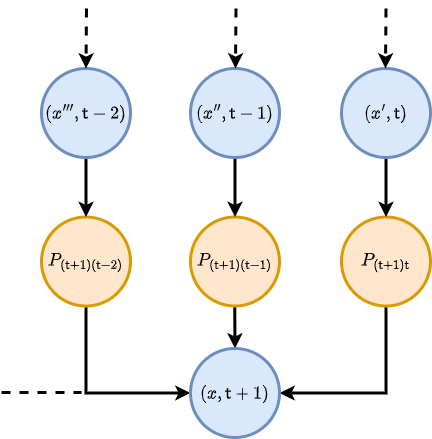
\includegraphics[width=8cm]{images/master-eq-graph.drawio.png}
\caption{Graph representation of Eq.~(\ref{eq:master-x-cont}).}
\label{fig:master-eqn}
\end{figure}

What if we wanted the joint distribution of both rows $P_{({\sf t}+1){\sf t}'}(x,x')$? One way to obtain this would be to extend Eq.~(\ref{eq:master-x-cont}) such that both matrix rows are marginalised over separately like so
%%
\begin{align}
&P_{({\sf t}+1){\sf t}'}(x,x') = \nonumber \\
&\qquad \frac{1}{({\sf t}'-1){\sf t}}\sum_{{\sf t}''=0}^{{\sf t}}\sum_{{\sf t}'''=0}^{{\sf t}'-1}\int_{\omega_{{\sf t}''}}{\rm d}x''\int_{\omega_{{\sf t}'''}}{\rm d}x''' P_{{\sf t}''{\sf t}'''}(x'', x''') P_{({\sf t}+1){\sf t}''}(x\vert x'')P_{{\sf t}'{\sf t}'''}(x'\vert x''') \label{eq:joint-master-x-cont} \,.
\end{align}
%%
Given Eqs.~(\ref{eq:master-x-cont}) and~(\ref{eq:joint-master-x-cont}) it's also possible to work out what the conditional probabilities would look like using the simple relation
%%
\begin{align}
P_{({\sf t}+1){\sf t}'}(x\vert x') &= \frac{P_{({\sf t}+1){\sf t}'}(x,x')}{P_{{\sf t}'}(x')} \label{eq:cond-master-x-cont} \,.
\end{align}
%%

The implicit notation in Eq.~(\ref{eq:master-x-cont}) can hide some staggering complexity. To analyse the system in more detail, we can also do a kind of Kramers-Moyal expansion~\cite{kramers1940brownian,moyal1949stochastic} for each point in time to approximate the overall equation like this
%%
\begin{align}
P_{{\sf t}+1}(x) &= \frac{1}{{\sf t}}\sum_{{\sf t}'=0}^{{\sf t}}P_{{\sf t}'}(x) - \frac{1}{{\sf t}}\sum_{{\sf t}'=0}^{{\sf t}}\sum_{i=1}^d\frac{\partial}{\partial x^i}\big[ \alpha^i_{({\sf t}+1){\sf t}'}(x)P_{{\sf t}'}(x)\big] \nonumber \\
& \qquad + \frac{1}{2{\sf t}}\sum_{{\sf t}'=0}^{{\sf t}}\sum_{i=1}^d\sum_{j=1}^d\frac{\partial}{\partial x^i}\frac{\partial}{\partial x^j}\big[ \beta^{ij}_{({\sf t}+1){\sf t}'}(x)P_{{\sf t}'}(x)\big] + \dots \label{eq:master-x-cont-kramers-moyal} \,,
\end{align}
%%
in which we have assumed that the state space is $d$-dimensional. In this expansion, we also needed to define these new integrals
%%
\begin{align}
\alpha^i_{({\sf t}+1){\sf t}'}(x) &=\int_{\omega_{{\sf t}'}} {\rm d}x'(x'-x)^iP_{({\sf t}+1){\sf t}'}(x'\vert x) \\
\beta^{ij}_{({\sf t}+1){\sf t}'}(x) &= \int_{\omega_{{\sf t}'}} {\rm d}x'(x'-x)^i(x'-x)^jP_{({\sf t}+1){\sf t}'}(x'\vert x) \,.
\end{align}
%%
So the matrix notation of Eq.~(\ref{eq:master-x-cont}) can indeed hide a very complicated calculation. Truncating the expansion at second-order, Eq.~(\ref{eq:master-x-cont-kramers-moyal}) tells us that there can be first and second derivatives contributing to the flow of probability to each element of the row $x=X_{{\sf t}+1}$ which depend on every element of the matrix $X'$. The probability does indeed \emph{flow}, in fact. We can define a quantity known as the `probability current' $J_{({\sf t}+1){\sf t}'}(x)$ from ${\sf t}'$ to $({\sf t}+1)$ which illustrates this through the following continuity relation
%%
\begin{align}
P_{{\sf t}+1}(x) - \frac{1}{{\sf t}}\sum_{{\sf t}'=0}^{{\sf t}}P_{{\sf t}'}(x) = \frac{1}{{\sf t}}\sum_{{\sf t}'=0}^{{\sf t}}\big[ P_{{\sf t}+1}(x) - P_{{\sf t}'}(x)\big] = - \frac{1}{{\sf t}}\sum_{{\sf t}'=0}^{{\sf t}}J_{({\sf t}+1){\sf t}'}(x) \,.
\end{align}
%%
By inspection of Eq.~(\ref{eq:master-x-cont-kramers-moyal}) we can therefore also deduce that
%%
\begin{align}
J^i_{({\sf t}+1){\sf t}'}(x) &= \alpha^i_{({\sf t}+1){\sf t}'}(x)P_{{\sf t}'}(x) - \frac{1}{2}\sum_{j=1}^d\frac{\partial}{\partial x^j}\big[ \beta^{ij}_{({\sf t}+1){\sf t}'}(x)P_{{\sf t}'}(x)\big] + \dots \,.
\end{align}
%%

What would happen if we assumed that $\alpha$ and $\beta$ were just arbitrary time-dependent functions? For example, let's make the following assumptions
%%
\begin{align}
\alpha^i_{({\sf t}+1){\sf t}'}(x) &= \mu^i({\sf t}')-x^i \\
\beta^{ij}_{({\sf t}+1){\sf t}'}(x) &= 2\Sigma^{ij}(\theta, {\sf t}') \,,
\end{align}
%%
where $\mu ({\sf t}')$ is an arbitrary vector-valued function of the timestep and $\Sigma (\theta ,{\sf t}')$ is an arbitrary matrix (often known as the `diffusion tensor') which depends on both the timestep and a set of hyperparameters $\theta$. If we now also assume stationarity of $P_{{\sf t}'}(x)=P_{{\sf t}''}(x)$ for any ${\sf t}'$ and ${\sf t}''$ such that
%%
\begin{align}
P_{{\sf t}+1}(x) = \frac{1}{{\sf t}}\sum_{{\sf t}'=0}^{{\sf t}} P_{{\sf t}'}(x) \,,
\end{align}
%%
we can solve Eq.~(\ref{eq:master-x-cont-kramers-moyal}) to obtain the following stationary solution
%%
\begin{align}
P_{{\sf t}'}(x) &= {\sf MultivariateNormalPDF}[x;\mu ({\sf t}'),\Sigma (\theta , {\sf t}')]\label{eq:stat-sol-kramers-moyal}\,.
\end{align}
%%
I actually hid a little bit of the detail in that last step; the solution also required the identification that the flow of probability between timesteps vanishes uniquely for each and every ${\sf t}'$ such that $J_{({\sf t}+1){\sf t}'}(x)=0$. 

\begin{figure}[h]
\centering
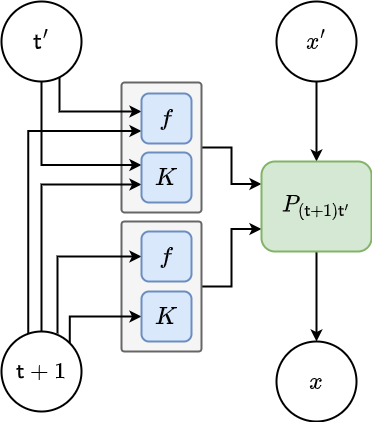
\includegraphics[width=8cm]{images/gp-like-diag.drawio.png}
\caption{Graph representation of the generative process implied by Eq.~(\ref{eq:stat-sol-kramers-moyal-cond}).}
\label{fig:stat-sol-kramers-moyal-cond}
\end{figure}

It's possible to take this derivation a bit further by expanding Eq.~(\ref{eq:joint-master-x-cont}) in a similar fashion, truncating it to second-order, assuming only time-dependent terms and then solving it in the stationary limit. By plugging this solution (and its corresponding marginal distribution equivalent) into Eq.~(\ref{eq:cond-master-x-cont}), it's possible to get something that looks like this conditional distribution
%%
\begin{align}
P_{({\sf t}+1){\sf t}'}(x\vert x') &\propto {\rm exp}\bigg\{ -\frac{1}{2}\sum^d_{i=1}\sum^d_{j=1}\big[ x-f({\sf t}+1)\big]^i [K^{-1}(\theta , {\sf t}+1,{\sf t}+1)]^{ij}\big[ x-f({\sf t}+1)\big]^j \nonumber \\
& \qquad \qquad + \sum^d_{i=1}\sum^d_{j=1}\big[ x-f({\sf t}+1)\big]^i [K^{-1}(\theta , {\sf t}+1,{\sf t}')]^{ij}\big[ x'-f({\sf t}')\big]^j  \bigg\} \label{eq:stat-sol-kramers-moyal-cond}\,,
\end{align}
%%
where $K(\theta , {\sf t}+1,{\sf t}')$ is some arbitrary covariance matrix that encodes how the correlation structure varies with the between compared states at two different timesteps and $K^{-1}(\theta , {\sf t}+1,{\sf t}')$ denotes taking its inverse. Eq.~(\ref{eq:stat-sol-kramers-moyal-cond}) may look a bit familiar to some readers who like using Gaussian processes from the machine learning literature~\cite{murphy2012machine} --- this version implies a \emph{generative} model for a future $x$ value (which we've illustrated in Fig~\ref{fig:stat-sol-kramers-moyal-cond}), in contrast to the more standard equation used to \emph{infer} values of $f$. These are two sides of the same coin though.

What other processes can be described by Eq.~(\ref{eq:master-x-cont})? For Markovian phenomena, the equation no longer depends on timesteps older than the immediately previous one, hence the expression reduces to just
%%
\begin{align}
P_{{\sf t}+1}(x) &= \int_{\omega_{\sf t}}{\rm d}x' P_{\sf t}(x') P_{({\sf t}+1){\sf t}}(x\vert x') \label{eq:master-x-cont-markov} \,.
\end{align}
%%
It's also easy to show that Eq.~(\ref{eq:master-x-cont-kramers-moyal}) naturally simplifies into the more usually applied Kramers-Moyal expansion when considering a Markovian process --- you just remove the sum over ${\sf t}'$ and the $1/{\sf t}$ normalisation factor. 

Note that an analog of Eq.~(\ref{eq:master-x-cont}) exists for discrete state spaces as well. We just need to replace the integral with a sum and the schematic would look something like this
%%
\begin{align}
P_{{\sf t}+1}(x) &= \frac{1}{{\sf t}}\sum_{{\sf t}'=0}^{\sf t}\sum_{\omega_{{\sf t}'}} P_{{\sf t}'}(x') P_{({\sf t}+1){\sf t}'}(x \vert x') \label{eq:master-x-disc} \,,
\end{align}
%%
where we note that the $P$'s in the expression above all now refer to \emph{probability mass functions}. Because the state space is now discrete, we cannot immediately intuit an approximative expansion from this expression. 

Ok, as a brief mathematical aside; if one is really determined to use a similar approach to the one we derived above, it's quite straightforward to rewrite it in terms of continuous-valued characteristic functions like so
%%
\begin{align}
\varphi_{{\sf t}+1}(s) &= \frac{1}{{\sf t}}\sum_{{\sf t}'=0}^{\sf t}\int_{\ell_{{\sf t}'}}{\rm d}s' {\cal C}(s') \varphi_{{\sf t}'}(s') \varphi_{({\sf t}+1){\sf t}'}(s \vert s') \label{eq:master-x-disc-char} \\
{\cal C}(s') &= \frac{1}{(2\pi )^d}\sum_{\omega_{{\sf t}'}}e^{-i(s'\cdot x')} \,,
\end{align}
%%
where $\ell_{{\sf t}'}$ defines all the continuous values that the vector $s'$ can possibly have at time ${\sf t}'$. In the expression above, ${\cal C}(s')$ acts like is a kind of comb\footnote{This is very similar to how a `Dirac comb' works in signal processing~\cite{brandwood2012fourier}.} to map the continuous frequency domain of $s'$ onto the discrete state space of $x'$. Note also that ${\cal C}(s')$ uses the imaginary number $i$ and, to be visually tidier, the dot product notation $a\cdot b$ just means the sum of vector elements: $a\cdot b = \sum_{\forall k}a^kb^k$. In principle, one can perform an approximative expansion on Eq.~(\ref{eq:master-x-disc-char}) like we did for continuous state spaces. This isn't always the most practical way of analysing the system though. 

We have one more important example to discuss and then we can cap off this analysis subsection. In the even-simpler case where $x$ is just a vector of binary `on' or `off' states, Eq.~(\ref{eq:master-x-disc}) reduces to
%%
\begin{align}
P^i_{{\sf t}+1} &= \frac{1}{{\sf t}}\sum_{{\sf t}'=0}^{\sf t} \sum_{j=1}^d P^j_{{\sf t}'} P^{ij}_{({\sf t}+1){\sf t}'} = \frac{1}{{\sf t}}\sum_{{\sf t}'=0}^{\sf t} \sum_{j=1}^d \big[ P^j_{{\sf t}'} A^{ij}_{({\sf t}+1){\sf t}'} + (1-P^j_{{\sf t}'}) B^{ij}_{({\sf t}+1){\sf t}'} \big] \label{eq:master-x-disc-binary}\,,
\end{align}
%% 
where $P^i_{{\sf t}'}$ now represents the probability that element $x^i=1$ (is `on') at time ${\sf t}'$. The matrices $A$ and $B$ are defined as conditional probabilities where the previous state in time $P^j_{{\sf t}'}$ was either `on' or `off', respectively.

\section{\sffamily Software design}

So we've proposed a computational formalism and done a bit of analysis on it to demonstrate that it can cope with a variety of different stochastic phenomena. Now we're ready to summarise what we want the stochadex software package to be able to do. But what's so complicated about Eq.~(\ref{eq:x-step-def})? Can't we just implement an iterative algorithm with a single function? It's true that the fundamental concept is very straightforward, but as we'll discuss in due course; the stochadex needs to have a lot of configurable features so that it's applicable in different situations. Ideally, the stochadex sampler should be designed to try and maintain a balance between performance and flexibility of utilisation.

If we begin with the obvious first set of criteria; we want to be able to freely configure the iteration function $F$ of Eq.~(\ref{eq:x-step-def}) and the timestep function $t$ of Eq.~(\ref{eq:t-steps-sum}) so that any process we want can be described. The point at which a simulation stops can also depend on some algorithm termination condition which the user should be able to specify up-front.

\begin{figure}[h]
\centering
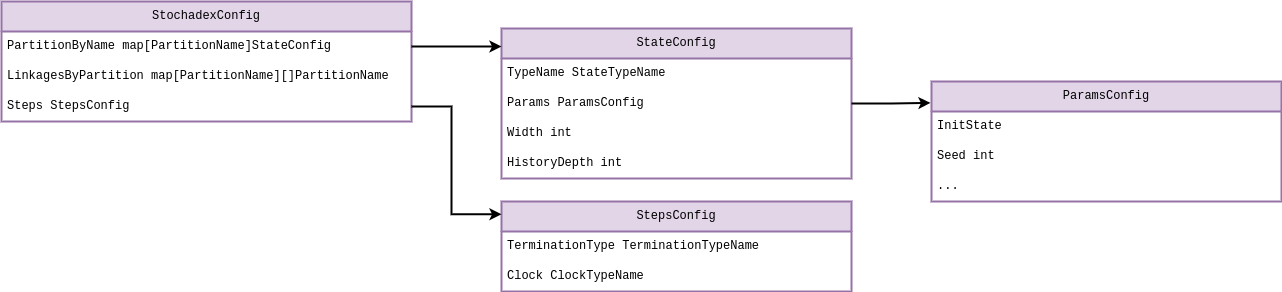
\includegraphics[width=13cm]{images/stochadex-data-types.drawio.png}
\caption{A relational summary of the core data types in the stochadex.}
\label{fig:data-types-design}
\end{figure}

Once someone has written the code to create these functions for the stochadex, we want to then be able to recall them in future only with configuration files while maintaining the possibility of changing their simulation run parameters. This flexibility should facilitate our uses for the simulation later in the book, and from this perspective it also makes sense that the parameters should include the random seed and initial state value.

The state history matrix $X$ should be configurable in terms of its number of rows --- what we'll call the `state width' --- and its number of columns --- what we'll call the `state history depth'. If we were to keep increasing the state width up to millions of elements or more, it's likely that on most machines the algorithm performance would grind to a halt when trying to iterate over the resulting $X$ within a single thread. Hence, before the algorithm or its performance in any more detail, we can pre-empt the requirement that $X$ should represented in computer memory by a set of partitioned matrices which are all capable of communicating to one-another downstream. In this paradigm, we'd like the user to be able to configure which state partitions are able to communicate with each other without having to write any new code.

For convenience, it seems sensible to also make the outputs from stochadex runs configurable. A user should be able to change the form of output that they want through, e.g., some specified function of $X$ at the time of outputting data. The times that the stochadex should output this data can also be decided by some user-specified condition so that the frequency of output is fully configurable as well. 

In summary, we've put together a schematic of data types and their relationships in Fig.~\ref{fig:data-types-design}. In this diagram there is some indication of the data type that we propose to store each piece information in (in Go syntax), and the diagram as a whole should serve as a useful guide to the basic structure of configuration files for the stochadex.

\begin{figure}[h]
\centering
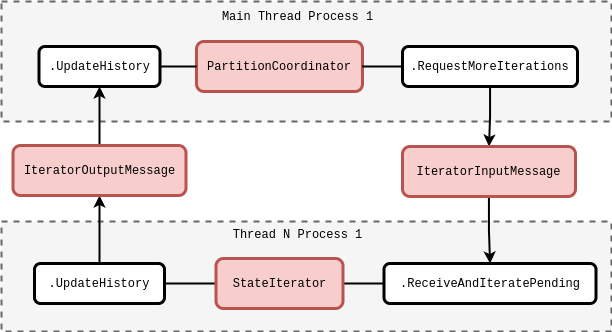
\includegraphics[width=13cm]{images/stochadex-loop.drawio.png}
\caption{A loop of the stochadex simulation algorithm with two state partitions.}
\label{fig:loop-design}
\end{figure}

It's clear that in order to simulate Eq.~(\ref{eq:x-step-def}), we need an interative algorithm which reapplies a user-specified function to the continually-updated history. But let's now return to the point we made earlier about how the performance of such an algorithm will depend on the size of the state history matrix $X$. The key bit of the algorithm design that isn't so straightforward is: how do we sucessfully split this state history up into separate partitions in memory while still enabling them to communicate effectively with each other? Other generalised simulation frameworks --- such as SimPy~\cite{simpy}, StoSpa~\cite{stospa} and FLAME GPU~\cite{flamegpu} --- have all approached this problem in different ways, and with different software architectures. 

In Fig.~\ref{fig:loop-design} we've illustrated what a loop involving separate state partitions looks like in the stochadex simulator. Each partition is handled by concurrently running execution threads of the same process, while a separate process may be used to handle the outputs from the algorithm. While this diagram illustrates only a single use for multiple processes, it's obviously true that we may run many of these whole diagrams at once on a multicore machine to generate a batch of independent ensembles if necessary.